\documentclass[11pt]{article}
\usepackage{geometry}
\usepackage{graphicx}
\usepackage{amssymb}
\usepackage{amsmath}
\usepackage{amsthm}
\usepackage{secdot}
\usepackage{booktabs}
\usepackage[numbers]{natbib}
\usepackage{hyperref}

\geometry{margin=1in,letterpaper} 
\newtheorem{thm}{Theorem}
\newtheorem{lem}{Lemma}
\newtheorem{problem}{Problem}


\newcommand\EE{\mathbb{E}}

\title{Sequence Bloom Trees for Large-Scale Search of Transcriptomic Read Sets}
\author{Brad Solomon and Carl Kingsford\\
Lane Center for Computational Biology, School of Computer Science,\\
Carnegie Mellon University, Pittsburgh, PA\\
bsolomo1@andrew.cmu.edu, carlk@cs.cmu.edu}
\date{}

\begin{document}
\maketitle
\begin{abstract}
We introduce the Sequence Bloom Tree data structure for efficiently indexing thousands of short-read sequencing experiments so that they can be searched by sequence. We apply Sequence Bloom Trees to the problem of finding conditions under which query genes are expressed. Our experiments are conducted on the entire set of 4,XXX publicly available RNA-seq experiments contained in the NIH Sequencing Read Archive for the breast, blood, and brain tissues, comprising XXX terabases of sequence. Sequence Bloom Trees of this size can be built using a single thread in XXX hours, and a query of 1000~nt can be searched in XXX seconds, over XXX times faster than fasta32. We also provide some theoretical guidance about appropriate parameter selection in Sequence Bloom Trees to trade off between search speed and accuracy. Sequence Bloom Trees allow for fast identification of experiments with expressed novel isoforms, even if these isoforms were unknown at the time the Sequence Bloom Tree was built. They are our first building block toward the goal of a highly searchable database of short-read sequencing data.
\end{abstract}

\section{Introduction}

% The motivation and introduction of the problem

The amount of DNA and RNA  short-read sequence data that has been published world-wide is huge. For example, the NIH's sequencing read archive~\cite{sra} alone contains 2,267,810,353,679,952 bases of sequence (about XXX~petabases). This collection of experiments could be a great resource understanding genetic variation, condition- and disease-specific gene function in ways the original depositors of the data did not anticipate. In aggregate too the data could provide the ability to answer questions  that a single experiment could not answer. However, its use is hampered by its size and the inability to search experiments by sequence. For example, a natural use of this data would exploit the XXX RNA-seq experiments to understand the conditions under which a novel or hypothesized alternatively spliced isoform $q$ is expressed by searching each SRA experiment for enough reads matching $q$ to indicate the $q$ was present in the experiment. cever, searching the entirety of such a database for expressed genes, novel isoforms, or homologous gene sequences  is not currently possible in reasonable computational time.  With this motivation, we define  the following search problem, which we will investigate below:
%
\begin{problem}\label{searchprob}
Given a query sequence $q$, which may be of any length, find the sequencing experiments that are likely to contain this sequence. If the experiment contains transcriptomic sequences, ``contains'' means likely expressed. If the experiment contains genomic or metagenomic sequences, ``contains'' means would be present in the assembled genomes.
\end{problem}

% why the problem is not yet solved / the challenges

Some progress has been made toward enabling sequence search on large databases.  The SRA does provide a sequence search functionality (SRA-BLAST~\cite{srablast}); however, this tool requires the selection of a small number of SRA experiments to which to restrict the search. Other similar services~\cite{othersrablast} limit the number of reads searched to XXX million (about XXX human RNA-seq  experiments, or XXX\% of the SRA). Existing full-text indexing data structures~\cite{fulltextindex} such as Borrows-Wheeler transform~\cite{BWT}, FM-index~\cite{fmindex}, compressed suffix arrays~\cite{comps}, or wavelet trees~\cite{wavelet} cannot at present be efficiently built at this scale, and do not directly support the search of millions of short sequences. Word-based indices~\cite{word1,word2}, such as those used by Internet search engines, are not appropriate for edit-distance-based biological sequence search. Sequence-specific solutions caBLAST~\cite{cablast} and caBLASTP~\cite{cablastp} have explored using custom compressed indices to speed up search. While successful at protein or genome search, they do not scale to collections of millions of short reads. All of these existing approaches do not handle the additional complication that a match to a query sequence $q$ may span many short reads.

% summary of results and their significance

We introduce a new indexing data structure called Sequence Bloom Trees (Figure~\ref{fig:schematic}) for application to sequence search. Sequence Bloom Trees allow for fast search of thousands of short-read sequencing experiments as required by Problem~\ref{searchprob}. They are practical to build and extremely efficient to search: building a SBT on XXX SRA experiments takes approximately XXX hours using a single thread on a single computer.  They are space efficient as well, requiring less than XXX\% of the space of the sequences they search. They are accurate, identifying XXX\% of truly matching sequencing experiments and with a false positive rate of $< XXX$\%.  They are easily distributed across computers in the cloud or a grid, and they are parallelizable when multiple cores are available. They are also dynamic, allowing insertions and deletions of new experiments, and progressive in the sense that a coarse-grained version of a Sequence Bloom Tree can be downloaded if needed and subsequently refined as more specific results are needed.

We apply Sequence Bloom Trees to the problem of searching RNA-seq experiments for expressed isoforms. We build a SBT on  all 4XX publicly available RNA-seq experiments in the SRA for the blood, breast, and brain tissues. Each of these tissues is among the top-5 most common tissues represented in the SRA. We use this SBT to search for tissue-specific expressed isoforms. We find that XXX. Sequence Bloom Trees have several natural parameters governing the tradeoff between index size, accuracy, and speed. We provide some theoretical guidance for setting these parameters to ensure the constructed SBTs perform well.

SBT represent a novel way to index large collections of short-read sequencing experiments to enable fast search by sequence. In addition to the application to RNA-seq reported here, we expect SBTs to be useful in the genomic and metagenomic contexts as well. They are our first step toward building a usable, high-performance searchable version of the petabases of sequence data in the SRA.

\section{The Bloom Tree Data Structure}

\subsection{Overview}
\begin{figure}
\centering
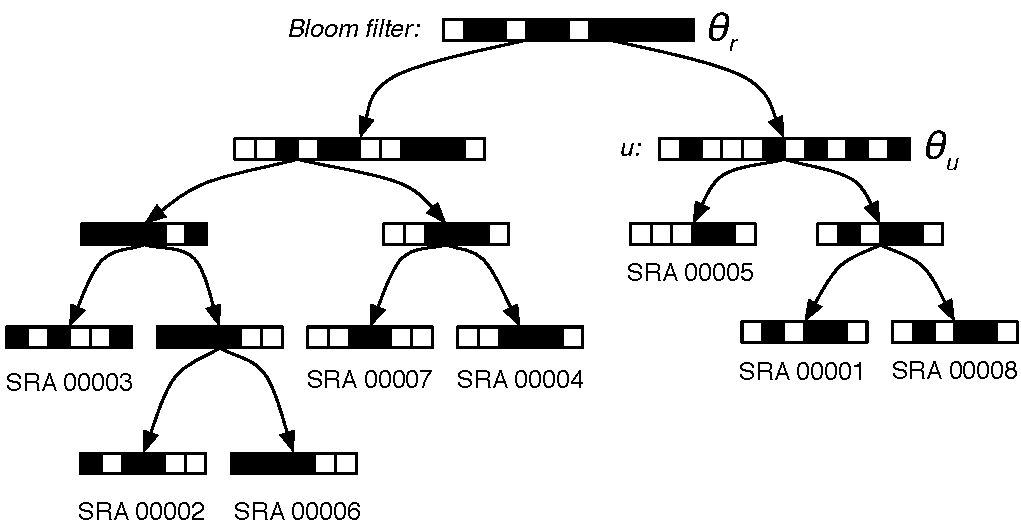
\includegraphics[width=0.7\textwidth]{BloomTreeSchematic}
\caption{Schematic of a Bloom Tree. Each node contains a bloom filter containing the kmers present in the sequencing experiments under it.}\label{fig:schematic}
\end{figure}

Sequence Bloom Trees are built around a collection of bloom filters~\cite{bloom,mitzenmacher}. Bloom filters are an efficient way to store a set of items from a universe $\mathcal{U}$. Each filter consists of a bit vector of length $m$ and a set of $h$ hash functions $h_i : \mathcal{U} \rightarrow [0,m)$ that map items to bits in the bit vector. Insertion of $u \in \mathcal{U}$ is performed by setting bits specified by $h_i(u)$ for $i = 1,\dots,h$ to 1. Querying for membership of $u$ checks these same bits; if they are all $1$, the filter is reported to contain $u$. Because of overlapping hash results, bloom filters have a one-sided error: they may report an item is present when it is not. This error can typically be made quite small by appropriate choice of $m$ and $h$. 

Sequence Bloom Trees (Figure~\ref{fig:schematic}) are trees in which the sequencing experiments are associated with leaves. Each node $v$ of the Sequence Bloom Tree contains a bloom filter that contains the set of kmers present in any read in any experiment in the subtree rooted at $v$. 

SBTs are different than cascading bloom filters~\cite{cascading}, which aim to reduce false positive rates of a single set query by recursively storing false positives in their own bloom filters.

The main challenge with scaling Sequence Bloom Trees to terabytes of sequence is saturation of the filters at levels of the tree near the root. The filter at any node $v$ is the union of the filters of its children. The union of bloom filters $b_1$ and $b_2$ can be efficiently computed by simply bitwise-OR of $b_1$ and $b_2$. However, this means as you move from the leaves to the root, the filters will tend to contain more and more bits set to $1$, increasing their false positive rate. This saturation can be overcome using several techniques: appropriate parameter selection, grouping of related experiments during insertion into the tree, and filter halving to efficiently support filters of varying size within the same tree. We describe these innovations below. Note that filters with poor false positive rates at high levels of the tree only affect query time: accuracy is governed entirely by the false positive rate of the leaf filters.

\subsection{Parameter selection}

Let $S$ be a collection of $r$ sequencing experiments with the property that each $s \in S$ contains $n$ distinct kmers, and where the probability that two different experiments $s_i$ and $s_j$ share any given kmer is $p$. In other words, the expected number of kmers that appear in $s_j$ that do not appear in $s_i$ is $d(1-p)$.

Further, let $F$ be a collection of $r$ bloom filters, each of length $m$, where $f_s \in F$ is the filter containing the kmers from  experiment $s \in S$. Assume each bloom filter employes $h$ hash functions.

\begin{lem}
Let $U = \bigcup_{f\in F} f$ be the union filter of the filters in $F$. The probability that a bit is not set in $U$ is
\begin{equation}\label{eqn:union}
\left(1 - \frac{1}{m}\right)^{hn\left(1+\sum_{i=1}^{r-1} (1-p)^i\right)} =
\left(1 - \frac{1}{m}\right)^{hn\left(1 - (1-p)^r\right)/p}
\end{equation}
In other words, the effective number of items in the union is $n(1-(1-p)^r)/p$.
\end{lem}
Equation~\ref{eqn:union} shows that when the overlap is large ($p$ is close to 0), the FPR of  $U$ approaches that of a single filter.

\begin{lem}
The  number of hashes for a union filter $U$ of $r$ filters that minimizes the FPR of $U$ is
\begin{equation}
h^* = (m (\ln 2) / (n(1-(1-p)^r)/p)) = 
(p\ln 2) / (1-(1-p)^r)\textit{load}).
\end{equation}
where $\textit{load} = n / m$.
Under this setting of $h$, the FPR of $U$ is 
\begin{equation}
\left(\frac{1}{2}\right)^{h^*},
\end{equation}
which is at most $1/2$ so long as $h^* \geq 1$.
\end{lem}
\begin{proof}
Follows directly by treating $U$ as a single filter containing $n(1-(1-p)^r)/p$ items.
\end{proof}

The case when $h^* < 1$  commonly occurs in practice when applying bloom trees because either the load of each filter is high or the overlap $p$ is low. While using fewer than 1 hash function is not possible, we can simulate having $h^* < 1$ effective hash functions  by randomly sampling only a $h^*$ fraction of the kmers that would be added to $U$ (i.e.\@ by adding a kmer to $U$ with probability $0 < h^* < 1$). This is possible here because when searching for a query string $Q$, we require many kmers of $Q$ to be present in the filter. The effect of omitting kmers due to random sampling therefore can be mitigated (up to a point) by lowering the  threshold $\theta$ of fraction of kmers that are required to be present  for the query to pass the filter.  Before we explore the appropriate setting of $\theta$, we look at the effect of the requirement of repeated queries on the FPR of a union bloom filter on a query string $Q$.


\begin{lem}\label{lem:query}
Let $Q$ be a query string containing $\ell$ distinct kmers. If we require that $>\lfloor\theta\ell\rfloor$ kmers appear in $U$ for $Q$ to pass the filter $U$ with FPR $f$, and if we treat the kmers of $Q$ as being independent, then the probability of a false positive pass through $U$ is
\begin{equation}\label{eqn:binom}
1 - \sum_{i=0}^{\lfloor \theta\ell\rfloor} \binom{\ell}{i}f^i(1-f)^{\lfloor\theta\ell\rfloor - i}. 
\end{equation}
The above expression is nearly $0$ when $f < \theta$.  
\end{lem}
\begin{proof}
Treating each kmer in $Q$ independently allows us to model the repeated queries using a binomial distribution, yielding~\eqref{eqn:binom}. A false positive in $Q$ occurs when $> \lfloor \theta \ell \rfloor$ false positive kmers occur in $U$. Let $X$ be the number of false positive kmers, and let $Y$ be the number of correctly determined kmers. Then
$\Pr[X > \theta\ell] = \Pr[Y \leq \ell - \theta\ell]$.
When $\theta \geq f$, we have $\ell - \theta\ell \leq \ell (1-f) = \EE[Y]$, and the following bound holds by Chernoff's inequality:
\begin{align}
\Pr[Y \leq \ell - \theta\ell] 
	&\leq \exp\left(\frac{-(\ell(1-f) - (\ell-\theta\ell))^2}{2(1-f)\ell}\right)\\
	&= \exp\left(\frac{-\ell(\theta - f)^2}{2(1-f)}\right)
\end{align}
\end{proof}

Lemma~\ref{lem:query} shows that so long as the $\theta$ is chosen to be greater than the FPR of $U$, very few false positive queries will pass the filter.

%1 - \sum = 1 - 2^theta * sum < 1 - 2^{theta ell} * 2^ell = 1 - 2^theta * ell^2

A scheme for sampling based on fraction hashes

-- approximation due to independence assumption

-- estimated number of nodes visited?

-- summary theorem about how to set h given a desired query FPR

\subsection{Query}

Given a query sequence $q$ and a Bloom Tree $T$, the sequencing experiments (at the leaves) that contain $q$ can be found by breaking $q$ into its constituent set of kmers $K_q$ and then flowing each of these kmers over $T$ starting from the root. At each node $u$, the bloom filter $b(u)$ at that node is queried for each of the kmers in $K_q$. If more than $\theta_u|K_s|$ kmers are reported to be present in $b(u)$, the search proceeds to all of the children of $u$, where $\theta_u$ is a node-specific cutoff between $0$ and $1$ governing the stringency required of the match. If fewer than that number of kmers is present, the subtree rooted at $u$ is not searched further (it is pruned). 

When a search proceeds to the children, the children are added to a queue for eventual processing.  Even though there may be a large frontier of nodes that are currently active, the memory usage for querying is the trivial amount of memory needed to store the tree topology and plus the memory needed to store the single current filter. If querying is parallelized in the natural way by having each thread pull an active frontier node off the single shared queue, the memory usage grows to a single filter per thread.

If several queries are to be made, they can be batched together so that a collection $\mathcal{C} = \{K_{q_1},\dots,K_{q_t}\}$ of queries starts at the root, and only queries for which $|b(u) \cap K_{q_i}| > \theta_u |K_{q_i}|$ are propagated to the children. When $\mathcal{C}$ becomes empty at a node, the subtree rooted at that node is pruned and not further searched.
The main advantage of batching queries in this way is locality of memory references. If $b(u)$ must be loaded from disk, it need be loaded only once per $\mathcal{C}$ rather than once per query. Batch queries can be parallelized in the same way as non-batched queries by storing with the nodes on the queue the indices of query sets that remain active at that node.

\subsection{Insertion}

% XXX: q vs Q
% XXX: ell is used twice for two different things

A Bloom Tree is built by repeated insertion. Given a Bloom Tree $T$, a new sequencing experiment $s$ can be inserted into $T$ by first computing the bloom filter $b(s)$ of the kmers present in $s$ and then walking from the root along a path to the leaves and inserting $s$ near the bottom of $T$ in the following way. When at node $u$, if $u$ has a single child, a node representing $s$ (and containing $b(s)$) is inserted as $u$'s second child. If  $u$ has two children, $b(s)$ is compared against the bloom filters $b(\ell(u))$ and $b(r(u))$ of the left $\ell(u)$ and right $r(u)$ children of $u$. The child with the more similar filter becomes the current node, and the process is repeated.  If $u$ has no children, $u$ represents a sequencing experiment $s'$. In this case, a new union node $v$ is created as a child of $u$'s parent. This new node has two children: $u$ and a new node representing $s$. 

As $s$ is walked down the tree, the filters at the nodes that are visited are unioned with $b(s)$. This unioning process can be made fast (and trivially paralelized for large filters) since the union of two bloom filters can be computed by ANDing together the bit vectors. This is particularly beneficial where GPU or vector computations can be used for these SIMD operations. 

This insertion process is designed to greedily group together sequencing experiments with similar bloom filters. This is important for two reasons. First, it helps to mitigate the problem of filter saturation. If too many dissimilar experiments are present under a node $u$, then $b(u)$ tends to have many bits set. In addition, by placing similar experiments in similar subtrees, more subtrees are pruned at an earlier stage of a query, reducing query time.

\subsection{Deletion}

Deletion proceeds from the to-be-deleted leaf $s$ up toward the root. Let $p(u)$ be the parent of any node $u$, and let $P_s$ be the path from $s$ to the root. We can assume that all the nodes along $P_s$ have two children (paths with nodes that have a single child can be compressed into a single node).  Assume  $s$ has a sibling $s'$. To delete $s$, the parent $p(s)$ is replaced by $s'$, and $p(p(s))$ has its filter recomputed as the union of $s'$ and its other child. We then walk up $P_s$, recomputing each filter as the union of its two child filters. This requires examining only $O(\text{depth}(s))$ filters. 

\subsection{Running times for insertion, deletion, and query}

Insertion and deletion both follow a single path from the root to a leaf $s$. In each case, two filters per examined node must be read in their entirety to either compute the similarity between the inserted filter and each node's 2 children, or to recompute the union when deleting. If the filters are of length $m$, the running time for insertion or deletion is $O(m\text{depth}(s))$.  Insertion can be made faster if sampling is used to compute the similarity between filters. In this case, $r$ random bits are compared between filters, reducing the running time for insertion to $O(r\text{depth}(s))$. Deletion can be made faster in practice by using lazy deletion: a node is initially only marked deleted and no filters are re-unioned. Once a large enough subtree rooted at $u$ has all of its nodes marked as deleted, the filters on $P_u$ are recomputed. 

The time for both insertion and deletion depends on the depth of the leaf being added or removed. If insertion and deletion are common, this depth can be reduced by creating a more balanced tree. The insertion procedure above favors grouping similar leaves over balance. A modified insertion scheme could favor inserting nodes into smaller subtrees by choosing the child to recurse into based on a combination of filter similarity and subtree size. We do not explore this alternative here as in our use case insertion is rare and deletion never occurs.

\subsection{Filter halving}

A central assumption of the preceding discussion is that the filter at each node is of the same length $m$. This allows for fast unioning during insertion or deletion. It has the downside, however, that the filter size must be chosen to be large enough so that filters closer to the root do not become saturated. This means that leaf filters have filters that are generally ``too large,'' wasting memory or, alternatively if a smaller filter size is used, the filters near the root become less useful to prune the search. This limitation can be overcome by using a standard bloom filter trick: the size of a filter can be efficiently halved. To do this, let $b_1$ and $b_2$ be the first $m/2$ and last $m/2$ bits of filter $b$, respectively.  Let $\{h_i\}$ be the hash functions for $b$. A filter $b'$ of length $m/2$ that contains the same items as $b$ can be created by $b' = b_1 \cap b_2$ and by then dropping the high-order bit from the output of each $\{h_i\}$.  Using this scheme, a large filter size $m$ can be chosen initially, and as nodes drop lower in the tree, their filters can be halved. 

%\left(1 - \frac{1}{m}\right)^{(\ln 2)m\left(1 - (1-p)^r\right)/p} \approx
%\left(\frac{1}{2}\right)^{\left(1 - (1-p)^r\right)/p}

\section{Computational Results}

\subsection{Selection of RNA-seq experiments}

\begin{table}
\centering
\begin{tabular}{lccc}
\toprule
Tissue & Number Experiments & Total Bases & Compressed FASTA Size \\
\midrule
Breast & \\
Brain & \\
Blood & \\
\midrule
Total & \\
\bottomrule
\end{tabular}
\caption{Sequencing experiments from the SRA used in the computational experiments here. These represent all the publicly accessible RNA-seq experiments for these tissues in the SRA.}
\end{table}

XXX: Describe how experiments were tagged with tissue (briefly), describe which were downloaded and why breast, brain, and blood were chosen. Summarize the size and reference table 1.

\subsection{Implementation}

The implementation used in the experiments below is in C++ and is available as open source at \url{http://www.cs.cmu.edu/~ckingsf/software/bloomtree}. Bitvectors were managed using the Succinct Data Structures Library~\cite{sdsl}. In the experiments below, a single thread was used to construct and search the tree. The filter sizes were chosen so that they have a FPR of $0.5$, resulting in a single hash function on filters of length $m=XXX$. Note that this is the FPR for a single kmer, not the FPR of the entire query. Theorem~\ref{lem:query} shows that even at this high filter FPR, the chance of a false positive for any query sequence of reasonable length (e.g.\@ $> 100$~nt) is very low. Filter halving was not used in these experiments. The cutoff $\theta$ was set to be the same for all nodes and was varied to assess the accuracy / time trade-off as described below.

\subsection{Query speed and accuracy}

- FPR
- TPR
- Fraction of leaf filters visited 
- Total fraction of tree visited
- Wallclock time

\subsection{Comparison to fasta32}

\subsection{Compression size}

\section{Discussion}

Bloom Trees have the additional advantage that they can be distributed over several computers in a cloud setting by having each computer manage a different subtree. In this setting, the insertion procedure should be modified to favor balanced distribution over computers.

If the set of sequencing experiments is relatively fixed, the filters at each node can be compressed using a data structure such as RRR~\cite{rrr} that allows $O(\log m)$ access to each bit within the filter. Early experiments with this approach indicated that query times do not increase significantly, but that unioning and the initial compression are slowed substantially.

A natural use case for Bloom Trees is that the tree could be built and stored at a central repository. Users who cannot store the entire Bloom Tree could download only the top levels as space allows, and run local queries on this subtree finding matching leaf nodes. Leaves in this subtree represent sets of sequencing experiments which could then be downloaded. Alternatively, only the subtrees of the Bloom Tree rooted at matching leaves could be downloaded and subsequently searched to find matching sequencing experiments.

\section*{Acknowledgements}

We would like to thank Geet Duggal for invaluable assistance annotating RNA-seq experiments with tissue type, and Guillaume Mar\c{c}ais for essential help modifying Jellyfish 2.0's bloom filter functionality to work with Bloom Trees. 

This work has been partially funded by the US National Science Foundation (CCF-1256087 and CCF-1053918) and US National Institutes of Health (R21HG006913 and R01HG007104). C.K. received support as an Alfred P. Sloan Research Fellow. 

\bibliographystyle{plainnat}
\bibliography{bloomtree}

\end{document}  